% =====================================================================
%  v1.5 — Intrinsic-Signal "Do-No-Harm" Gating for a Frozen-Base
%  Soft-Prompt Memory Wrapper.
%  Self-contained technical note: ALL settings + ALL metric definitions
%  (black-box / benchmark-native AND intrinsic, incl. per-layer) with
%  interpretation. Plan 08, mem-X line. Created 2026-06-04.
%  Compile: pdflatex v1.5-intrinsic-gating-study-2026-06-04.tex
% =====================================================================
\documentclass[11pt]{article}
\usepackage[margin=1in]{geometry}
\usepackage{amsmath,amssymb}
\usepackage{booktabs}
\usepackage{array}
\usepackage{graphicx}
\usepackage{longtable}
\usepackage{xcolor}
\usepackage[colorlinks=true,linkcolor=blue,urlcolor=blue]{hyperref}
\usepackage{microtype}

\newcommand{\OURS}{\textsc{Wrap}}
\newcommand{\GIST}{\textsc{Gist}}
\newcommand{\noctx}{\texttt{no\_context}}
\newcommand{\fullctx}{\texttt{full\_context}}
\newcommand{\code}[1]{\texttt{#1}}

\title{\textbf{Intrinsic-Signal ``Do-No-Harm'' Gating for a Frozen-Base
Soft-Prompt Memory Wrapper}\\[2pt]
\large Settings, Metric Definitions, and a Signal--Usefulness
Correlation Study (v1.5)}
\author{Plan 08 (mem-X line) --- internal technical note}
\date{2026-06-04}

\begin{document}
\maketitle

\begin{abstract}
v1 of this project showed that a learned $K$-token soft-prompt memory
wrapper around a \emph{frozen} LLM is a \emph{narrow lossy compressor}:
it matches the Gist-Tokens baseline on QuALITY but \emph{negatively
transfers} on benchmarks it never trained for (verbatim retrieval,
multi-hop QA), sometimes scoring \emph{below} the base model with no
wrapper at all. Because the whole point of a frozen base is that adding
a module should not \emph{lose} points, v1.5 asks: can we \emph{gate}
the wrapper's intervention --- suppress it when it would hurt --- using
cheap signals computable at inference? This note fixes \textbf{all
experimental settings} (\S\ref{sec:settings}) and \textbf{all metric
definitions} (\S\ref{sec:metrics}), both the benchmark-native black-box
outcomes and the intrinsic signals (including \emph{per-layer} logit-lens
quantities), then reports the first correlation study
(\S\ref{sec:results}) identifying \emph{which} intrinsic signals --- and
at \emph{which layers} --- predict the benchmark's own usefulness
measure. The design principle: first learn what correlates with the
target, then design the gate around it.
\end{abstract}

\tableofcontents

% =====================================================================
\section{Deliverables and source links}
\label{sec:deliverables}

This PDF is the compiled v1.5 technical note. The links below are the
source-of-truth entry points for the deliverables, facts, and main result
summaries around Plan 08.

\subsection{v1 wrapper facts and main result}
\begin{itemize}
\item \textbf{Settings registry:}
\href{https://github.com/BDeMo/research-notes/blob/main/notes/plans/08-model-outputs-delta-w/settings/settings.md}{settings.md}.
Every result cell in this report should trace to a setting ID; v1
headline cells use \textbf{P08-S2}, and v1.5 signal-grid cells use
\textbf{P08-S3}.
\item \textbf{Main v1 result summary:}
\href{https://github.com/BDeMo/research-notes/blob/main/notes/plans/08-model-outputs-delta-w/v1-results-2026-06-03.md}{v1-results-2026-06-03.md}.
This is the main facts document for the \code{mem-embedding} wrapper,
including the three-regime transfer law.
\item \textbf{v1 pivot / lessons:}
\href{https://github.com/BDeMo/research-notes/blob/main/notes/plans/08-model-outputs-delta-w/v1-if-wrapper-doesnt-work-2026-06-03.md}{v1-if-wrapper-doesnt-work-2026-06-03.md}.
This explains why v1 is framed as a characterization paper and how it
leads to v1.5.
\item \textbf{History / chronology:}
\href{https://github.com/BDeMo/research-notes/blob/main/notes/plans/08-model-outputs-delta-w/v0-how-we-got-here.md}{v0-how-we-got-here.md}.
\end{itemize}

\subsection{v1.5 signal grid and gating deliverables}
\begin{itemize}
\item \textbf{Compiled report:}
\href{https://github.com/BDeMo/research-notes/blob/main/notes/plans/08-model-outputs-delta-w/summary/2026-06-04/v1.5-intrinsic-gating-study-2026-06-04.pdf}{v1.5-intrinsic-gating-study-2026-06-04.pdf}.
\item \textbf{LaTeX source:}
\href{https://github.com/BDeMo/research-notes/blob/main/notes/plans/08-model-outputs-delta-w/summary/2026-06-04/v1.5-intrinsic-gating-study-2026-06-04.tex}{v1.5-intrinsic-gating-study-2026-06-04.tex}.
\item \textbf{Signal-grid folder:}
\href{https://github.com/BDeMo/research-notes/tree/main/notes/plans/08-model-outputs-delta-w/raw/grids-2026-06-04}{grids-2026-06-04}.
\item \textbf{Main signal-ranking figures:}
\href{https://github.com/BDeMo/research-notes/blob/main/notes/plans/08-model-outputs-delta-w/raw/grids-2026-06-04/rank_help.png}{rank\_help.png}
and
\href{https://github.com/BDeMo/research-notes/blob/main/notes/plans/08-model-outputs-delta-w/raw/grids-2026-06-04/rank_interesting.png}{rank\_interesting.png}.
\item \textbf{Signal-grid CSVs:}
\href{https://github.com/BDeMo/research-notes/blob/main/notes/plans/08-model-outputs-delta-w/raw/grids-2026-06-04/grid_auroc_correct.csv}{grid\_auroc\_correct.csv},
\href{https://github.com/BDeMo/research-notes/blob/main/notes/plans/08-model-outputs-delta-w/raw/grids-2026-06-04/grid_auroc_noharm.csv}{grid\_auroc\_noharm.csv},
\href{https://github.com/BDeMo/research-notes/blob/main/notes/plans/08-model-outputs-delta-w/raw/grids-2026-06-04/grid_spearman_cont.csv}{grid\_spearman\_cont.csv},
\href{https://github.com/BDeMo/research-notes/blob/main/notes/plans/08-model-outputs-delta-w/raw/grids-2026-06-04/corr_long.csv}{corr\_long.csv}.
\end{itemize}

\subsection{v2 and idea table}
\begin{itemize}
\item \textbf{v2 plan:}
\href{https://github.com/BDeMo/research-notes/blob/main/notes/plans/08-model-outputs-delta-w/v2-plan.md}{v2-plan.md}.
\item \textbf{v2 related work:}
\href{https://github.com/BDeMo/research-notes/blob/main/notes/plans/08-model-outputs-delta-w/v2-related-work.md}{v2-related-work.md}.
\item \textbf{Q2 activation-memory probe:}
\href{https://github.com/BDeMo/research-notes/blob/main/notes/plans/08-model-outputs-delta-w/q2-activation-memory-probe.md}{q2-activation-memory-probe.md}.
\item \textbf{Plan table:}
\href{https://github.com/BDeMo/research-notes/blob/main/notes/plans/README.md}{notes/plans/README.md}.
\item \textbf{Full idea table:}
\href{https://github.com/BDeMo/research-notes/blob/main/notes/ideas/README.md}{notes/ideas/README.md},
including H6 (Plan 08) and related follow-ups H3/H7/G4/G5.
\item \textbf{Original brainstorm:}
\href{https://github.com/BDeMo/research-notes/blob/main/notes/ideas/inference-time-training.md}{inference-time-training.md}.
\end{itemize}

% =====================================================================
\section{Experiments: what was run, what is running, what is planned}
\label{sec:experiments}

\subsection{Compute environment}
Three Kubernetes pods (shared, multi-tenant): \texttt{sam-dev-test}
($1{\times}$H200-143GB), \texttt{sam-dev-ray} ($4{\times}$H100-80GB),
\texttt{sam-dev} ($4{\times}$H100-80GB). Qwen3-8B is present on all
three; Qwen3-14B only on \texttt{sam-dev}. Each probe run trains one
wrapper (one seed) on a single GPU and evaluates all assigned
benchmarks; seeds are sharded one-per-GPU to use the cluster in
parallel. All runs use the memory-safe probe (\code{scripts/probe\_v2.py}):
last-position hidden states are cloned and the full activation tensors
freed, a single encoder pass is taken per chunk, and the CUDA cache is
flushed periodically --- a fix introduced after an out-of-memory
postmortem on the 80\,GB cards (retained all-position
\code{hidden\_states} views $+$ redundant encoder passes).

\subsection{Runs ledger}
\begin{center}\footnotesize
\setlength{\tabcolsep}{4pt}
\begin{tabular}{l l l c c p{3.0cm} l}
\toprule
run & setting & purpose & seeds & $n$/bench & benchmarks & status\\
\midrule
Phase 0 & P08-S3 & prediction-derived signals, free-gen scored & 4--5 & 800 & QuALITY, MuSR, RULER, Hotpot, Trivia, SQuAD, MARCO & done (\S\ref{sec:phase0})\\
seed-42 probe & P08-S3 & native-MC $+$ 37-layer signals (single seed) & 1 & 150 & QuALITY, MuSR, RULER, Hotpot, Trivia & done (\S\ref{sec:seed42})\\
9-seed extended & P08-S3 & full battery, multi-seed (robust) & 9 & 1350 & QuALITY, MuSR, RULER, Hotpot, Trivia & \textbf{done} (\S\ref{sec:multiseed})\\
new-bench (8B) & P08-S3 & 4 more answer-type angles & 5 & 150 & QuALITY-hard, SQuAD-v2, NarrativeQA, MS-MARCO & running (seed42 done) \\
14B cross-scale & P08-S3 & does the signal hold at $2{\times}$ scale? & --- & --- & main 5 & deferred (pod busy)\\
gate (Phase 4) & P08-S4 & input-conditioned do-no-harm gate & --- & --- & public-only & planned (\S\ref{sec:gate-target})\\
\bottomrule
\end{tabular}
\end{center}
The robust conclusions (\S\ref{sec:multiseed}) rest on the
\emph{9-seed extended} run; Phase 0 and seed-42 are earlier, smaller
passes kept for traceability and because seed-42 illustrates the
granularity effect (and one single-seed artifact the 9-seed run
corrects).

\subsection{Probe protocol (per eval item)}
On the frozen base we run: (i) the \textbf{wrapper} (memory prefix $+$
query) with hidden-state output; (ii) \textbf{\noctx{}} (query only);
(iii) a \textbf{memory-ablation} pass (wrapper prompt with attention to
the $K$ memory tokens masked) for the causal-influence signal; (iv)
greedy generation for wrapper and \noctx{}; (v) for MC benchmarks,
per-option log-likelihood scoring; (vi) a teacher-forced pass over the
wrapper's own generated answer for answer-span statistics. From these we
log the native black-box outcome (\S\ref{sec:native}) and the full
intrinsic battery across granularities and angles
(\S\ref{sec:intrinsic}) --- $\sim$6--10 forward passes per item,
$\sim$50 GPU-min per seed for five benchmarks at $n{=}150$.

% =====================================================================
\section{Settings}
\label{sec:settings}

Unless a table states otherwise, numeric signal/correlation results in
this report use setting
\href{https://github.com/BDeMo/research-notes/blob/main/notes/plans/08-model-outputs-delta-w/settings/settings.md#p08-s3--v15-intrinsic-signal-probe}{P08-S3}.
The underlying wrapper recipe is
\href{https://github.com/BDeMo/research-notes/blob/main/notes/plans/08-model-outputs-delta-w/settings/settings.md#p08-s1--v1-canonical-wrapper-recipe}{P08-S1};
v1 three-regime background comparisons use
\href{https://github.com/BDeMo/research-notes/blob/main/notes/plans/08-model-outputs-delta-w/settings/settings.md#p08-s2--v1-phase-y-three-regime-benchmark-cells}{P08-S2}.

\subsection{Frozen base and the wrapper}
The base $f_\theta$ is \textbf{Qwen3-8B} (hidden size $d=4096$, $36$
decoder layers), \emph{frozen} throughout; only the wrapper trains. The
wrapper $\phi_\psi$ ($\approx 218$M trainable params, $2.67\%$ of the
base) maintains a memory state $m_t\in\mathbb{R}^{K\times d}$, $K=32$.

\paragraph{Write side (recurrence).} For each context chunk $c_t$
($t=1{:}N$, $N=6$ chunks of $\le 256$ tokens), a single Perceiver-IO
cross-attention$+$FFN block $g_\phi$ (heads $h=8$, FFN mult $2$,
$L=1$ layer) produces a candidate, and the wrapper exposes the residual:
\begin{equation}
\Delta m_t = \mathrm{LN}\!\big(g_\phi(m_{t-1},c_t)-m_{t-1}\big),
\qquad
m_t = m_{t-1} + \alpha_{\mathrm{upd}}\cdot \Delta m_t,
\end{equation}
with $\alpha_{\mathrm{upd}}$ a learned scalar (init $1.0$). $\Delta m_t$
is published on \code{MemoryState.extra["last\_delta"]} for geometry
probes.

\paragraph{Read side (combine).} At query time the final memory $m_T$ is
delivered to the base. The canonical mode is \code{xattn}: a second
cross-attention lets memory re-read the raw chunk pool
$H_{\mathrm{chunks}}$, then the refined memory is prepended as a soft
prefix:
\begin{equation}
m_T' = m_T + \alpha_{\mathrm{ro}}\cdot
\mathrm{LN}\!\big(\mathrm{CrossAttn}(m_T,H_{\mathrm{chunks}})\big),
\qquad
\text{inputs\_embeds} = [\,m_T';\, x\,],
\end{equation}
where $x$ are the query-token embeddings. Seven combine modes exist
(\code{prefix}, \code{residual}, \code{interleave}, \code{hybrid},
\code{xattn}, \code{xattn\_residual}, \code{gated}); only \code{gated}
is unimplemented and is the \emph{target} of v1.5
(\S\ref{sec:gate-target}). No combine mode ever moves a base weight.

\paragraph{Answer head (auxiliary, training only).} For categorical
training tasks a $\mathrm{Linear}(d,n_{\mathrm{cls}})$ head on
$\mathrm{pool}(m_T)$ supplies a direct class-prediction gradient that
bypasses the frozen base.

\paragraph{Joint training loss.}
\begin{equation}
\mathcal{L} = \mathcal{L}_{\mathrm{CE}}
+ \lambda_{\mathrm{kl}}\,\mathrm{KL}(p_{\mathrm{student}}\Vert p_{\mathrm{teacher}})
+ \lambda_{\mathrm{div}}\,\tfrac{1}{T-1}\!\sum_t \cos(\Delta m_t,\Delta m_{t-1})
+ \lambda_{\mathrm{ah}}\,\mathcal{L}_{\mathrm{ah}},
\end{equation}
teacher $=$ same base reading the full context (\fullctx{}).

\subsection{Training recipe (locked)}
\begin{center}\small
\begin{tabular}{llll}
\toprule
knob & value & knob & value\\
\midrule
base & Qwen3-8B (frozen, bf16) & combine & \code{xattn}\\
$K$ (memory tokens) & 32 & $h$ heads / $L$ layers & 8 / 1\\
train dataset & \code{categorical\_niah} & $N$ train items & 500\\
$N$ chunks & 6 & max chunk tokens & 256\\
optimiser & AdamW, lr $3\!\times\!10^{-5}$, const & steps & 1800 (SFT)\\
$\lambda_{\mathrm{kl}}$ & 1.0 & $\lambda_{\mathrm{div}}$ & 0.1\\
$\lambda_{\mathrm{ah}}$ (answer head) & 0.5 & seeds & \{42,7,11,13,1,5,17,99,23\}\\
\bottomrule
\end{tabular}
\end{center}

\subsection{Evaluation protocol}
The wrapper is trained \emph{only} on \code{categorical\_niah} and
evaluated \textbf{zero-shot} on public benchmarks via a
\code{--eval-dataset} flag (wrapper weights never updated on eval data).
For every eval item we run, on the same frozen base:
(i) the \textbf{wrapper} (memory prefix $+$ query); and
(ii) \textbf{\noctx{}} (query only) --- which \emph{is} the base
\emph{without} the wrapper, since the wrapper replaces the document with
$K$ memory tokens. \noctx{} is therefore the do-no-harm reference
(\S\ref{sec:usefulness}). We also have the standard baselines
\fullctx{} (base reads the full document), \code{retrieval} (BM25 top-2
chunks), \code{summary}.

\paragraph{Compute fan-out.} The probe (\code{scripts/probe\_v2.py})
trains one wrapper per seed and evaluates all 5 benchmarks with full
instrumentation. Seeds are sharded one-per-GPU across 8 GPUs
(\code{sam-dev-test} H200 $\times$1; \code{sam-dev-ray} H100 $\times$4;
\code{sam-dev} H100 $\times$4) to produce a multi-seed dataset.

\subsection{Benchmarks}
\label{sec:benchmarks}
All are public long-context QA, evaluated zero-shot. ``Answer space''
drives the native metric (\S\ref{sec:native}).
\begin{center}\small
\begin{tabular}{lllr l}
\toprule
benchmark & source & answer space & $n_{\mathrm{eval}}$ & native metric\\
\midrule
QuALITY      & Pang et al.\ 2022      & 4-way MC (A--D)     & 150 & accuracy (likelihood)\\
MuSR-mm      & Sprague et al.\ 2024   & MC (murder myst.)   & 150 & accuracy (likelihood)\\
RULER-NIAH   & Hsieh et al.\ 2024     & 6-digit value       & 150 & contains-recall\\
HotpotQA     & Yang et al.\ 2018      & free-form span      & 150 & SQuAD EM/F1\\
TriviaQA-RC  & Joshi et al.\ 2017     & span $+$ aliases    & 150 & EM/F1 (max over aliases)\\
SQuAD v2     & Rajpurkar et al.\ 2018 & span / no-answer    & --- & EM/F1 ($+$abstain)\\
NarrativeQA  & Ko\v{c}isk\'y et al.\ 2018 & open-ended       & --- & ROUGE-L, BLEU\\
MS MARCO     & Bajaj et al.\ 2016     & free-form          & --- & ROUGE-L, BLEU-1\\
\bottomrule
\end{tabular}
\end{center}

% =====================================================================
\section{Metric definitions}
\label{sec:metrics}

We separate three families: (a) the benchmark-\emph{native} black-box
\emph{outcome} metrics (\S\ref{sec:native}); (b) the \emph{usefulness}
labels derived from them, which are what a gate should track
(\S\ref{sec:usefulness}); and (c) the \emph{intrinsic signals} that are
candidate gate \emph{inputs} (\S\ref{sec:intrinsic}).

\subsection{Black-box (benchmark-native) outcome metrics}
\label{sec:native}
\textbf{Principle: score by the benchmark's own method.} Notably, the
multiple-choice benchmarks are natively scored by \emph{likelihood}, not
free-form generation; our earlier free-generation $+$ letter-parsing
under-counted the base (e.g.\ \fullctx{} appeared as $0.079$ on QuALITY
purely as a parsing artifact).

\paragraph{(MC) Length-normalised option log-likelihood.}
For options $o^{(1)},\dots,o^{(C)}$ with token sequences
$o=(o_1,\dots,o_{|o|})$, score each by the mean log-prob of its
continuation given the prompt $P$:
\begin{equation}
s(o)=\frac{1}{|o|}\sum_{i=1}^{|o|}\log p_\theta\!\big(o_i\mid P,o_{<i}\big),
\qquad
\widehat{o}=\arg\max_o s(o),\quad
\mathrm{acc}=\mathbf{1}[\widehat{o}=o^\star].
\end{equation}
We also record the continuous \emph{margin}
$\;\mathrm{mc\_margin}=s(o^\star)-\max_{o\ne o^\star}s(o)\;$ and the
gold log-prob $s(o^\star)$ --- richer (less noisy) targets than binary
accuracy at $n{=}150$.

\paragraph{(span) SQuAD EM / F1.} With SQuAD normalisation
$\mathcal{N}(\cdot)$ (lowercase; strip punctuation; drop articles
\{a,an,the\}; collapse whitespace):
\begin{equation}
\mathrm{EM}=\mathbf{1}[\mathcal{N}(\hat y)=\mathcal{N}(y)],\qquad
\mathrm{F1}=\frac{2\,\mathrm{prec}\cdot\mathrm{rec}}{\mathrm{prec}+\mathrm{rec}},
\end{equation}
on the multiset of normalised tokens; over a reference/alias set $R$ the
score is $\max_{y\in R}$ (TriviaQA aliases, NarrativeQA refs). HotpotQA
sup-fact/joint metrics are \emph{not} applicable (the wrapper predicts
no supporting facts). SQuAD~v2: a no-answer item scores $1$ iff the model
abstains; our current harness restricts to answerable items
(SQuAD-1.1-style) --- an open gap.

\paragraph{(retrieval) RULER contains-recall.}
$\;\mathrm{em\_value}=\mathbf{1}[\,y \subseteq \hat y\,]\;$ (the planted
6-digit value appears in the output; official \code{acc\_match\_str\_any}).

\paragraph{(generation) ROUGE-L / BLEU.} ROUGE-L is the LCS-based F-score
$\tfrac{2 P_{\mathrm{lcs}}R_{\mathrm{lcs}}}{P_{\mathrm{lcs}}+R_{\mathrm{lcs}}}$,
$P_{\mathrm{lcs}}=\mathrm{LCS}(\hat y,y)/|\hat y|$,
$R_{\mathrm{lcs}}=\mathrm{LCS}(\hat y,y)/|y|$; BLEU-$n$ is the
brevity-penalised geometric mean of clipped $n$-gram precisions. Both
taken max/over the reference set. ROUGE-L is the reported headline for
NarrativeQA and MS MARCO.

\subsection{Usefulness labels (the gate's target) and reference}
\label{sec:usefulness}
Let $u_w$ be the wrapper's native correctness on an item and $u_b$ the
reference's. We define per item:
\begin{align*}
\texttt{correct} &= \mathbf{1}[u_w \ge \tau] \quad(\tau{=}0.5),\\
\texttt{noharm}  &= \mathbf{1}[u_w \ge u_b],\\
\texttt{help} &= \mathbf{1}[u_w{>}\tau \wedge u_b{\le}\tau],\quad
\texttt{hurt} = \mathbf{1}[u_w{\le}\tau \wedge u_b{>}\tau],\\
\texttt{cont} &= \text{continuous target (MC: } \mathrm{mc\_margin};\ \text{else native value)}.
\end{align*}
\textbf{Two references.} Against \noctx{} (base without wrapper) the
wrapper is already harmless on $80$--$100\%$ of items per benchmark
(\S\ref{sec:results}); the damaging gap is against \fullctx{}
(compression discards usable context). Hence the gate is best understood
as a \emph{compressibility detector}: decide when lossy memory is safe
vs.\ when to fall back to more context. The \emph{ideal} gate maximises
\texttt{noharm} (never drop below the base) while keeping \texttt{help}.

\subsection{Intrinsic signals (candidate gate inputs)}
\label{sec:intrinsic}
All are computed at inference without the gold label. Let the wrapper
run produce final-token next-token distribution $p_w$ and per-layer
last-token hidden states $h_\ell^{w}$ ($\ell=0{:}36$); the \noctx{} run
gives $p_0$, $h_\ell^{0}$.

\paragraph{Final-layer signals.}
Entropy $H(p)=-\sum_v p_v\log p_v$; confidence $\mathrm{conf}=\max_v p_v$;
margin $=p_{(1)}-p_{(2)}$ (top-two gap); divergence
$\mathrm{kl\_w0}=\mathrm{KL}(p_w\Vert p_0)$; agreement
$\mathbf{1}[\arg\max p_w=\arg\max p_0]$. Reported as \code{entropy\_w},
\code{conf\_w}, \code{margin\_w}, \code{kl\_w0}, \code{first\_tok\_agree}.

\paragraph{Per-layer logit-lens signals (the multi-layer probe).} Project
each layer's last-token hidden through the frozen final norm and
unembedding $W_U$ to get an early ``readout'' distribution:
\begin{equation}
\pi_\ell = \mathrm{softmax}\!\big(W_U\,\mathrm{LN}_f(h_\ell)\big).
\end{equation}
From $\pi_\ell^{w}$ we record \code{ll\_entropy\_w\_l}, \code{ll\_conf\_w\_l},
\code{ll\_margin\_w\_l}; the wrapper-vs-base divergence
$\mathrm{\code{ll\_kl\_wb\_l}}=\mathrm{KL}(\pi_\ell^{w}\Vert\pi_\ell^{0})$;
and the depth-stabilisation flag
$\mathrm{\code{ll\_argmax\_agree\_final\_l}}=\mathbf{1}[\arg\max\pi_\ell^{w}
=\arg\max p_w]$. We also record per-layer \emph{hidden drift}
\begin{equation}
\mathrm{\code{drift\_l}} =
\frac{\lVert h_\ell^{w}-h_\ell^{0}\rVert_2}{\lVert h_\ell^{0}\rVert_2+\epsilon},
\end{equation}
i.e.\ how much the wrapper perturbs each layer's residual stream at the
answer position. \textbf{Rationale (the multi-layer hypothesis):}
different depths encode different things --- early-layer drift may flag
format perturbation (harmful), mid-layer $\pi_\ell$ agreement-with-base
may flag safe compression, late-layer confidence may flag correctness ---
so the most predictive signal need not live at the final layer, and a
\emph{per-layer} gate can read whichever layer carries the signal.

\paragraph{Memory geometry.} $\mathrm{drift\_mem}=\lVert m_T-m_0\rVert_F$;
$\mathrm{delta\_mean}=\tfrac1N\sum_t\lVert\Delta m_t\rVert$;
$\mathrm{q\_chunk\_cos}=\cos(\overline{\mathrm{enc}}(q),\overline{\mathrm{enc}}(c))$
(query vs.\ chunk mean-pooled encodings; max and mean over chunks).

\paragraph{Ensemble signals (Phase 0 only; not purely intrinsic).}
\code{intervene\_vs\_noctx} $=\mathbf{1}[\hat y_w\ne\hat y_0]$;
\code{agree\_retrieval} $=\mathbf{1}[\hat y_w=\hat y_{\mathrm{retr}}]$;
\code{n\_baselines\_agree} $=\#\{$baselines whose prediction $=\hat y_w\}$;
\code{w\_outlen} (generated length). These need running other strategies
and so are candidate \emph{ensemble} gate inputs.

\subsection{Correlation metrics}
\label{sec:corr}
For each (signal, layer) we report \textbf{AUROC} against a binary label
(rank statistic: $\mathrm{AUROC}=\Pr[s_{+}>s_{-}]$; $0.5=$ no signal,
$|{\cdot}-0.5|$ measures discriminative power, $<0.5$ means the signal is
\emph{inversely} predictive), and \textbf{Spearman} $\rho$ against the
continuous target. A \emph{per-layer profile} reports, per layer-metric,
the layer maximising $|\mathrm{AUROC}-0.5|$. A planned multivariate
logistic probe on the full $\{$metric$\times$layer$\}$ vector estimates
the achievable gate ceiling.

% =====================================================================
\section{Results and interpretation}
\label{sec:results}

Setting for all result cells in this section:
\href{https://github.com/BDeMo/research-notes/blob/main/notes/plans/08-model-outputs-delta-w/settings/settings.md#p08-s3--v15-intrinsic-signal-probe}{P08-S3},
unless explicitly labeled as v1 three-regime background
(\href{https://github.com/BDeMo/research-notes/blob/main/notes/plans/08-model-outputs-delta-w/settings/settings.md#p08-s2--v1-phase-y-three-regime-benchmark-cells}{P08-S2}).

\paragraph{Status.} The \textbf{9-seed multi-seed study
($n{=}1350$/bench) is complete} and is the robust result
(\S\ref{sec:multiseed}); it \emph{supersedes} the single-seed seed-42
rankings (\S\ref{sec:seed42}) and corrects one of them. Seed-42 tables
are kept for traceability and because they illustrate the granularity
effect.

\subsection{Phase 0 --- base rates (free-gen scored, $5{,}600$ items)}
\label{sec:phase0}
Setting for every cell in this table: P08-S3.
\begin{center}\small
\begin{tabular}{l rrr rrr}
\toprule
bench & $u_w$ & \noctx{} & \fullctx{} & help\% & hurt\% & noharm\%\\
\midrule
quality    & 0.193 & 0.141 & 0.079 & 13 & 8  & 92\\
musr\_mm   & 0.492 & 0.494 & 0.551 & 11 & 12 & 89\\
trivia\_qa & 0.168 & \textbf{0.338} & 0.565 & 3 & \textbf{20} & 80\\
hotpot\_qa & 0.086 & 0.104 & 0.438 & 3 & 5  & 95\\
ruler\_niah& 0.000 & 0.000 & 0.994 & 0 & 0  & 100\\
\bottomrule
\end{tabular}
\end{center}
\noindent\textbf{Read:} vs.\ \noctx{} the wrapper is mostly harmless
(noharm $80$--$100\%$); it \emph{actively} hurts only on TriviaQA
($20\%$). The catastrophe is vs.\ \fullctx{} (RULER $0.994\!\to\!0$,
Hotpot $0.44\!\to\!0.09$) --- compression discards usable context. So
the gate is a compressibility detector, not a corruption filter.

\subsection{Seed-42 gate signal sheet (native-MC + per-layer)}
\label{sec:seed42}
Setting for every cell in this subsection: P08-S3 (single-seed slice).
\begin{center}\small
\begin{tabular}{l l l r l}
\toprule
bench & native metric & best intrinsic signal & AUROC & predictive layer\\
\midrule
hotpot\_qa & squad\_f1        & \code{conf\_w}        & \textbf{0.753} & near-final (34--35)\\
quality    & accuracy (LL)    & \code{ll\_kl\_wb@30}  & \textbf{0.680} & \textbf{mid-layer 30}\\
trivia\_qa & squad\_f1        & \code{ll\_conf@34}    & \textbf{0.653} & layer 34\\
musr\_mm   & accuracy (LL)    & \code{ll\_entropy@11} & 0.582          & weak (at chance)\\
ruler\_niah& exact\_value     & ---                   & ---            & undefined ($0$ correct)\\
\bottomrule
\end{tabular}
\end{center}

\paragraph{Per-layer profile} (layer maximising $|\mathrm{AUROC}-0.5|$
for \texttt{correct}; bold $=$ best per row):
\begin{center}\small
\begin{tabular}{l rrrr}
\toprule
signal & quality & hotpot & trivia & musr\\
\midrule
\code{ll\_kl\_wb\_l}            & \textbf{@30: 0.680} & @34: 0.332 & @33: 0.284 & @34: 0.555\\
\code{ll\_conf\_w\_l}          & @30: 0.353 & \textbf{@35: 0.731} & \textbf{@34: 0.653} & @22: 0.428\\
\code{ll\_margin\_w\_l}        & @30: 0.333 & @35: 0.696 & @34: 0.630 & @19: 0.422\\
\code{drift\_l}                & @2: 0.374  & @33: 0.397 & @26: 0.370 & @17: 0.531\\
\code{ll\_argmax\_agree\_final\_l} & @34: 0.461 & @34: 0.597 & @23: 0.343 & @34: 0.479\\
\bottomrule
\end{tabular}
\end{center}

\subsection{Interpretation}
\begin{enumerate}
\item \textbf{The wrapper's own confidence/margin predicts correctness}
on the QA benchmarks (\code{conf\_w}/\code{ll\_conf} AUROC $0.65$--$0.75$).
A confidence-thresholded gate is therefore viable: low confidence
$\Rightarrow$ suppress the wrapper.
\item \textbf{The predictive layer is benchmark-dependent and often not
the final one.} QuALITY's strongest signal is logit-lens KL-vs-base at
\emph{layer 30} (\code{ll\_kl\_wb@30}$=0.680$), whereas Hotpot/Trivia
peak at layers 34--35. This empirically validates the multi-layer
hypothesis: a single-layer (output-only) gate would miss the QuALITY
signal; a per-layer gate has the right information to read.
\item \textbf{Where there is no signal, the gate should simply close.}
MuSR is at chance (max AUROC $0.58$) and RULER is uniformly wrong
(AUROC undefined). These are exactly the regimes where the wrapper must
defer to context; a do-no-harm gate that closes there is correct, not a
failure.
\item \textbf{Ensemble signals are stronger but costlier} (Phase 0:
\code{n\_baselines\_agree} AUROC $0.83$--$0.90$ on extractive benches),
trading deployability for accuracy --- a fallback if intrinsic signals
prove insufficient under multi-seed.
\end{enumerate}

\subsection{Multi-seed result (9 seeds, $n{=}1350$/bench) --- robust}
\label{sec:multiseed}
Setting for every cell in this subsection: P08-S3 (robust 9-seed slice).
Pooling seeds $\{42,7,11,13,1,5,17,99,23\}$ with the full extended
battery sharpens and \emph{corrects} the single-seed picture.
\begin{center}\small
\begin{tabular}{l l l r r}
\toprule
bench & best signal & angle & AUROC & Spearman\\
\midrule
trivia\_qa  & \code{seq\_logprob}  & confidence & \textbf{0.769} & $+0.357$\\
            & \code{ll\_kl\_wb@34} & divergence & 0.229 (inv.)   & $-0.40$\\
hotpot\_qa  & \code{top5\_mass\_w} & confidence & \textbf{0.761} & $+0.316$\\
quality     & (none robust)        & ---        & $\le 0.55$     & ---\\
musr\_mm    & (none)               & ---        & $\le 0.52$     & ---\\
ruler\_niah & undefined            & ---        & ---            & ---\\
\bottomrule
\end{tabular}
\end{center}
\begin{enumerate}
\item \textbf{Wrapper output confidence robustly predicts correctness}
on extractive QA (\code{seq\_logprob}/\code{top5\_mass\_w}, AUROC
$0.76$--$0.77$); the cheapest granularity (output/span) wins, and
per-layer \code{ll\_conf} aggregates add only a little (trivia: final
$0.60\!\to\!$max $0.66$).
\item \textbf{Wrapper$\to$base divergence is inversely predictive}
(\code{ll\_kl\_wb},\,\code{kl\_0w},\,\code{js},\,\code{tv}): a larger
distribution shift $\Rightarrow$ the wrapper is more likely
\emph{wrong} (trivia \code{ll\_kl\_wb@34} $\rho{=}{-}0.40$). A natural
gate input, used inversely.
\item \textbf{The single-seed QuALITY ``layer-30 KL'' peak ($0.68$,
\S\ref{sec:seed42}) was an artifact} --- it falls to $\approx 0.47$ at
9 seeds. No intrinsic signal robustly predicts QuALITY correctness;
this is exactly why the multi-seed study was necessary.
\item \textbf{Where there is no signal (musr/ruler), the gate should
close} (do no harm) --- the correct behaviour, not a failure.
\end{enumerate}
\noindent\textbf{Gate input (decided):} wrapper output \emph{confidence}
$+$ wrapper$\to$base \emph{divergence} (inverse), both robust at
$n{=}1350$; per-layer features are secondary inputs to the multivariate
probe.

% =====================================================================
\section{Signal codebook: setting, definition, and rationale}
\label{sec:codebook}
\textbf{Setting for every correlation in this report.} Each signal is
computed in the per-item probe protocol of \S\ref{sec:experiments}, on a
\emph{frozen} Qwen3-8B with the wrapper trained zero-shot on
\code{categorical\_niah} (\S\ref{sec:settings}; setting
\href{https://github.com/BDeMo/research-notes/blob/main/notes/plans/08-model-outputs-delta-w/settings/settings.md#p08-s3--v15-intrinsic-signal-probe}{P08-S3}).
The rankings of
\S\ref{sec:interesting} are pooled over \textbf{9{,}750 items across 9
benchmarks} (main five at 9 seeds, new four at 5 seeds); targets
\code{help} (wrapper correct $\wedge$ base wrong), \code{noharm}
(wrapper $\ge$ base) and \code{lift} are as in \S\ref{sec:usefulness};
AUROC/Spearman as in \S\ref{sec:corr}. ``Pass'' = which forward(s) the
signal reads. AUROC${<}0.5$ = \emph{inverse} predictor.

\subsection{Confidence / uncertainty angle (obvious --- removed in \S\ref{sec:interesting})}
\begin{center}\footnotesize\begin{tabular}{p{3.0cm} p{3.9cm} p{6.0cm}}
\toprule signal & pass / setting & why it relates (and why it is obvious)\\ \midrule
\code{conf\_w}, \code{margin\_w}, \code{entropy\_w}, \code{top5\_mass\_w} & first generated-token distribution, wrapper run & model self-confidence; a sharp/low-entropy distribution $\Rightarrow$ correct. The ``model is sure $\Rightarrow$ right'' calibration effect. (\code{top5\_mass\_w} is the top \code{help} predictor, AUROC 0.653.)\\
\code{span\_entropy\_*}, \code{span\_conf\_mean}, \code{seq\_logprob}, \code{perplexity} & teacher-forced pass over the wrapper's own greedy answer & the same confidence, aggregated over the whole answer span rather than one token.\\
\code{conf\_0}, \code{entropy\_0}, \code{margin\_0} & \noctx{} run (base, query only) & \emph{item difficulty}: if the base is confident with no context, the item is easy and the wrapper is unlikely to make it worse. (\code{entropy\_0} is the top \code{noharm} predictor, AUROC 0.646.)\\
\code{ll\_\{conf,margin,entropy\}\_w\_l} & logit-lens of the wrapper hidden state, per layer & depth-resolved confidence.\\
\bottomrule\end{tabular}\end{center}

\subsection{Divergence-from-base angle (interesting)}
\begin{center}\footnotesize\begin{tabular}{p{3.0cm} p{3.9cm} p{6.0cm}}
\toprule signal & pass / setting & why it relates (non-obviously)\\ \midrule
\code{kl\_w0}, \code{kl\_0w}, \code{js\_w0}, \code{tv\_w0} & first-token distribution, wrapper \emph{vs} \noctx{} & how far the memory moves the base's \emph{output} distribution; a large move means the wrapper is overriding the base's prior, and empirically that override is usually wrong (inverse).\\
\code{ll\_kl\_wb\_l@$\ell$} & logit-lens KL between wrapper and \noctx{} hidden at layer $\ell$ & deviation of the base's \emph{internal} representation at depth $\ell$. Mid--late layers ($\ell{\approx}25$--34) are where the answer decision forms; large KL there = the memory is fighting the base's own reasoning $\Rightarrow$ harm. The strongest non-obvious correlate.\\
\code{mem\_influence\_kl}, \code{mem\_influence\_argmax\_change} & wrapper run \emph{vs} the same run with attention to the $K$ memory tokens masked & causal: how much the base actually \emph{uses} the memory. Double-edged (genuine use vs.\ wrong override).\\
\bottomrule\end{tabular}\end{center}

\subsection{Representation-geometry angle (interesting)}
\begin{center}\footnotesize\begin{tabular}{p{3.0cm} p{3.9cm} p{6.0cm}}
\toprule signal & pass / setting & why it relates (non-obviously)\\ \midrule
\code{drift\_l@$\ell$}, \code{drift\_l::late} & $\lVert h_\ell^{w}{-}h_\ell^{0}\rVert/\lVert h_\ell^{0}\rVert$ at the answer position, per layer & raw magnitude by which the soft prompt perturbs the residual stream. A pure geometry quantity, yet mid--late perturbation predicts harm: gentle steering helps, violent distortion hurts.\\
\code{drift\_mem} & $\lVert m_T{-}m_0\rVert_F$ of the recurrence & total movement of the memory state from its learned init; encodes ``how much was written'' but explodes on collapse.\\
\code{delta\_mean/max/last/trend} & per-chunk $\lVert\Delta m_t\rVert$ over the recurrence & shape of the write process; \code{delta\_trend} (growing vs.\ decaying updates) distinguishes a recurrence that \emph{integrates} from one that \emph{chases} each chunk.\\
\code{slot\_norm\_\{mean,std,max\}}, \code{slot\_active\_frac} & per-slot magnitudes of $m_T$ & how many of the $K$ memory slots are actually used; a degenerate (few-active) memory encodes less.\\
\bottomrule\end{tabular}\end{center}

\subsection{Relevance and agreement angles}
\begin{center}\footnotesize\begin{tabular}{p{3.0cm} p{3.9cm} p{6.0cm}}
\toprule signal & pass / setting & why it relates\\ \midrule
\code{q\_chunk\_\{max,mean\}\_cos}, \code{q\_chunk\_spread} & cosine of mean-pooled query vs.\ chunk encodings (encoder) & a \emph{data}-side property: whether the query semantically matches a chunk, i.e.\ whether the answer-bearing content was even available for the memory to encode. Non-obvious because it ignores the model entirely.\\
\code{first\_tok\_agree} & wrapper vs \noctx{} argmax (first token) & whether the memory changed the base's answer at all; no change $\Rightarrow$ safe, change $\Rightarrow$ intervention (risky). Borderline-obvious.\\
\code{ll\_argmax\_agree\_final\_l} & layer-$\ell$ logit-lens argmax $=$ final argmax & decision-crystallisation depth: how early the answer stabilises.\\
\bottomrule\end{tabular}\end{center}

% =====================================================================
\section{Filtering to the non-obvious correlates}
\label{sec:interesting}
The strongest correlates of correctness are unsurprising --- the
wrapper's own \emph{confidence} (\code{top5\_mass\_w} AUROC $0.653$ for
\code{help}; \code{entropy\_0} $0.646$ for \code{noharm}). These are
``model-is-sure $\Rightarrow$ model-is-right'' and carry little design
insight. \textbf{Dropping the entire confidence angle} leaves $151$
signals; only \textbf{11} still clear
$|\mathrm{AUROC}_{\text{help}}{-}0.5|\ge 0.10$, and they cluster into a
single coherent, non-obvious story
(Fig.~\ref{fig:interesting}):
\begin{itemize}
\item \textbf{Mid--late-layer wrapper$\leftrightarrow$base divergence}
(\code{ll\_kl\_wb\_l@25}--\code{34}, peak $\ell{=}30$,
$\mathrm{AUROC}_{\text{help}}{\approx}0.36$, \emph{inverse}): the more
the memory bends the base's \emph{internal} distribution at the layers
where the decision forms, the less likely it helps. Not a confidence
signal --- a \emph{representational-conflict} signal.
\item \textbf{Mid--late-layer residual-stream drift}
(\code{drift\_l@24}--\code{35}, $\mathrm{AUROC}_{\text{help}}{\approx}0.40$,
inverse): the raw magnitude by which the soft prompt perturbs the late
hidden state predicts harm --- a pure-geometry quantity with no obvious
tie to correctness.
\item \textbf{Layer-localised}: early-layer KL/drift is \emph{not}
predictive (mere format perturbation); the signal lives specifically in
the decision-forming mid--late band ($\ell{\approx}25$--34).
\end{itemize}
\noindent\textbf{Reading.} The design-relevant, non-obvious signal is
``\emph{is the memory fighting the base's own late-layer reasoning?}''
(divergence / drift at $\ell{\approx}30$), used \emph{inversely}: high
conflict $\Rightarrow$ suppress. A naive confidence threshold would miss
exactly this, which is what makes it interesting for the gate.

\begin{figure}[h]\centering
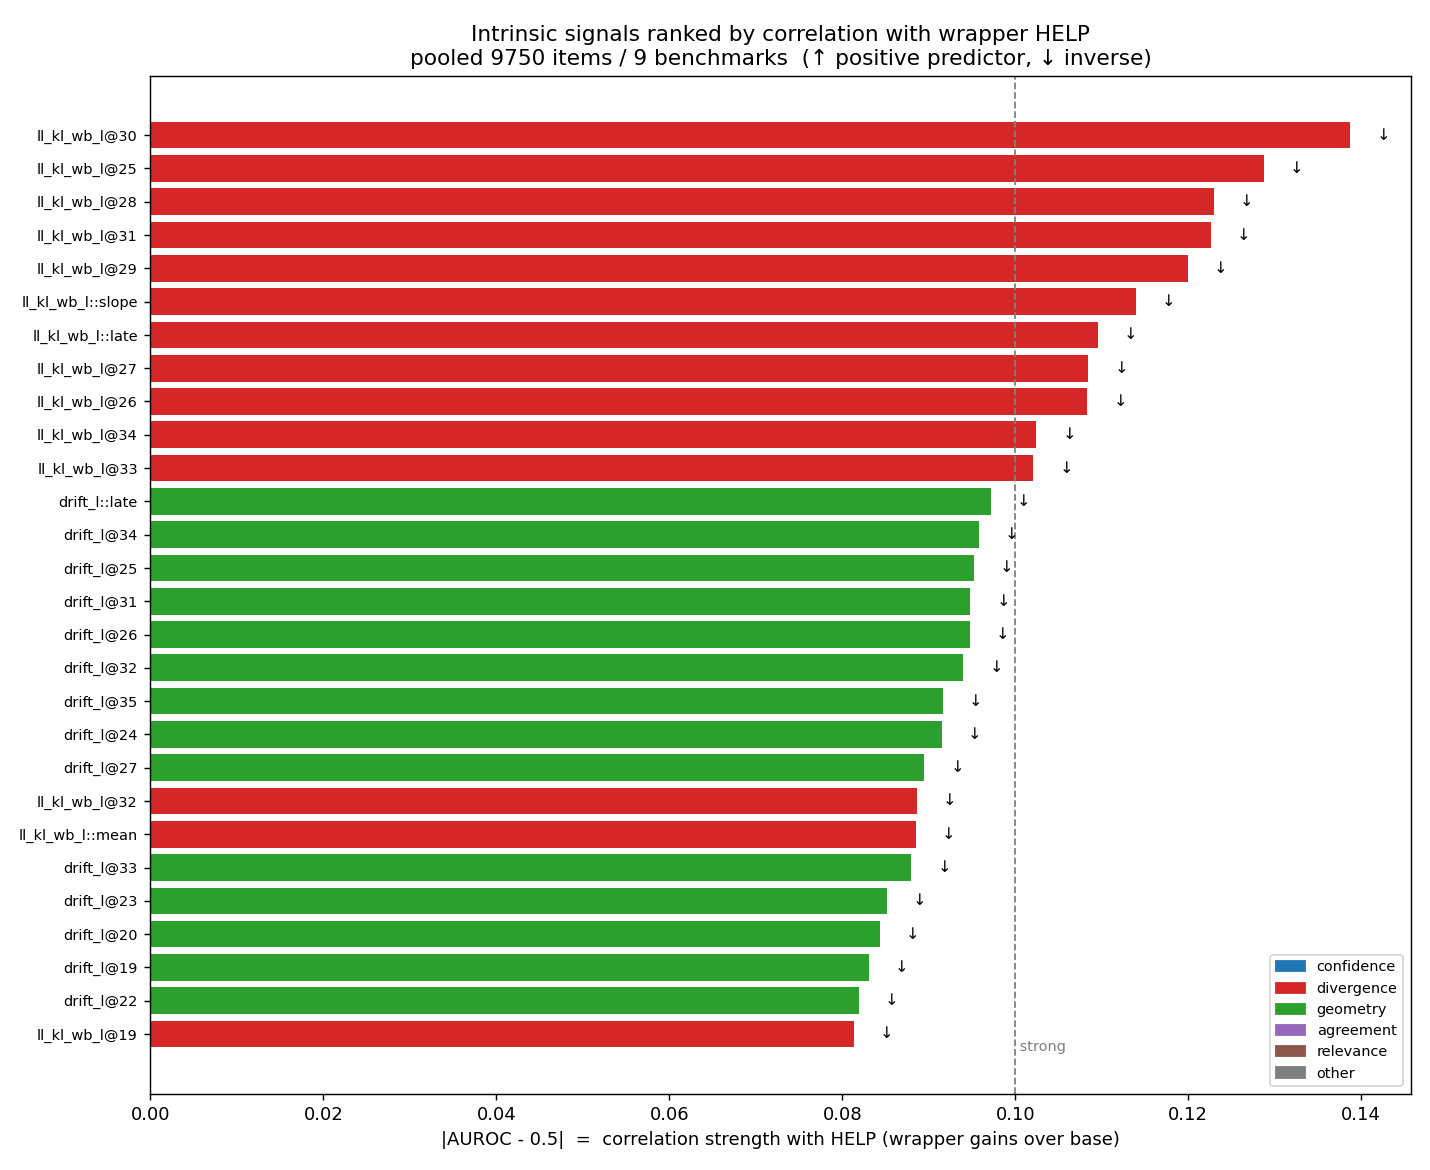
\includegraphics[width=0.9\linewidth]{../../raw/grids-2026-06-04/rank_interesting.png}
\caption{Non-obvious correlates of wrapper \code{help} (confidence angle
removed), pooled $9{,}750$ items over $9$ benchmarks, high$\to$low by
$|\mathrm{AUROC}{-}0.5|$ ($\downarrow$ = inverse predictor). The
survivors are mid--late-layer divergence (\code{ll\_kl\_wb}) and
residual drift (\code{drift\_l}).}
\label{fig:interesting}
\end{figure}

% =====================================================================
\section{The gate target and next steps}
\label{sec:gate-target}

\paragraph{Mechanism.} Implement the placeholder \code{gated} combine as
an input-conditioned convex mix, optionally \emph{per base layer} $\ell$:
\begin{equation}
e_t' = (1-g_\ell)\,e_t + g_\ell\,\tilde m_{t,\ell},
\qquad
g_\ell = \sigma\!\big(w_\ell^\top \phi_\ell(\text{signals}) + b_\ell\big),
\quad b_\ell \ll 0,
\end{equation}
so $g_\ell\!\approx\!0$ at init (wrapper $\approx$ identity, base
preserved; cf.\ LLaMA-Adapter zero-init gating, Flamingo $\tanh$-gating,
DISeL input-conditioned LoRA gating). The gate reads the signals the
correlation study selects (likely late-layer \code{conf}/\code{ll\_conf}
for correctness $+$ mid-layer \code{ll\_kl\_wb} for compressibility).

\paragraph{Training the gate.} On \code{categorical\_niah} $+$ decoy
items (irrelevant context $\Rightarrow$ gate should close, target $=$
base \noctx{} output) plus a do-no-harm KL regulariser
$\mathrm{KL}(p_{\mathrm{wrap}}\Vert p_{\mathrm{base}})$ on held-out
OOD-like text. \textbf{Eval public-only}; success $=$ Regime-A gain
retained \emph{and} \code{OURS\_gated} $\ge$ \noctx{} on Regime-B/C.

\paragraph{Pending.} (i) Multi-seed bands ($9$ seeds) to firm up
\S\ref{sec:results}. (ii) Multivariate logistic probe for the gate
ceiling. (iii) Multi-layer injection (only if the per-layer profile's
payoff over output-only justifies it).

% =====================================================================
\section*{Pointers}
\begin{itemize}\setlength\itemsep{1pt}
\item Probe: \code{mem-embedding/scripts/probe\_v2.py} (train$+$save,
native-MC, $37$-layer logit-lens/drift).
\item Analysis: \code{scripts/signal\_corr.py}; Phase 0
\code{scripts/signal\_study.py}.
\item Live ledger: \code{mem-embedding/summary/matrix.md} (v1 archived in
\code{matrix-archive-2026-06-03.md}).
\item Native metrics impl: \code{llm-infra/src/llm\_infra/benchmark\_metrics.py}.
\item Runs: \code{runs/pv2-20260604-181915UTC} (seed 42),
\code{runs/pv2-seed*-20260604-*UTC} (multi-seed).
\end{itemize}

\end{document}
